\section{Ringoszillator}
In diesem Teil des Versuches soll ein Ringoszilloskop untersucht werden.
\subsection{Experimentelle Durchf\"uhrung}
In Abbildung 4 ist ein Ringoszilloskop aus f\"unf Invertern dargestellt. Dies wurde mit Hilfe eines CMOS-Bausteines \textbf{Typ: 74HC04} aufgebaut. Um das Signal zu messen wird dies mit einem weiteren Inverter entkoppelt.
\begin{figure}[!h]
\begin{center}
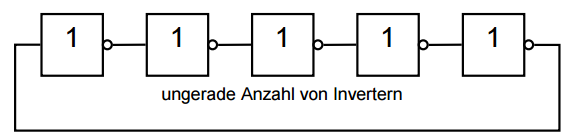
\includegraphics[scale=0.5]{bild/Ringoszillator}
\caption{Schaltung eines Ringoszillator}
\end{center}
\end{figure} 
\subsection{Ergebnisse und Diskussion}
\begin{figure}[!h]
\begin{minipage}[t]{0.5\textwidth}
\includegraphics[width=\textwidth]{bild/Inverter5V}
\end{minipage}
\hfill
\begin{minipage}[t]{0.5\textwidth}
\includegraphics[width=\textwidth]{bild/Inverter4V}
\end{minipage}
\caption{Ausgangssignal bei U$_{\text{DD}}$~$=$~5~$V$ bzw. 4~$V$}
\end{figure}
%%%%%%%%%%%%%%%%%%%%%%%%%%%%%%%%%%%%%%%%%%%%%%%%%%%%%%%%%
\begin{figure}[!h]
\begin{minipage}[t]{0.5\textwidth}
\includegraphics[width=\textwidth]{bild/Inverter3V}
\end{minipage}
\hfill
\begin{minipage}[t]{0.5\textwidth}
\includegraphics[width=\textwidth]{bild/Inverter2V}
\end{minipage}
\caption{Ausgangssignal bei U$_{\text{DD}}$~$=$~3~$V$ bzw. 2~$V$}
\begin{center}
\begin{minipage}[t]{0.5\textwidth}
\includegraphics[width=\textwidth]{bild/Inverter1V}
\end{minipage}
\caption{Ausgangssignal bei U$_{\text{DD}}$~$=$~1~$V$}
\end{center}
\end{figure}
